\chapter{Ausblick}
Diese Arbeit hat gezeigt, dass die Datenanalyse in der Wissenschaft durch den Einsatz relationaler Datenbanksysteme verbessert werden kann. Bestehende Bash-Skripte, die bislang bei der Analyse den Vorzug erhalten haben, können automatisiert in SQL übersetzt werden, den Grundstein hierfür hat diese Arbeit gelegt.
Der vorgestellte Übersetzer parst die Bash-Syntax bis auf Funktionen und kann grundlegende Kommandos in SQL übersetzen. Bei der Weiterentwicklung des Übersetzers sollte in Erwägung gezogen werden einen AST (abstrakter Syntaxbaum) explizit zu generieren, sodass die Übersetzungslogik vom Parsen unabhängig ist.
Außerdem hat die Arbeit durch die Implementierung des TPC-H Skriptes verfügbare Skripte geliefert, die bei Weiterentwicklungen eines Übersetzers als Testdaten dienen können.
\section{Schleifen}
Bisher wurde nicht mit Schleifen experimentiert. Da eine Schleife immer als Ganzes eingelesen wird, führt dies zu Problemen, da zuerst die Kommandos im Rumpf bearbeitet werden, am Ende die Schleife selber. Bisher regelte dies eine globale Variable, die speichert, in welcher Ebene sich das Kommando befindet. Dies sollte bei zukünftigen Entwicklungen verbessert werden.

\section{Sprache awk separat}
Im Moment erfolgt das Parsen von awk-Ausdrücken innerhalb der Bash-Grammatik, obwohl diese grundverschieden sind, so spielen in awk Leerräume keine Rolle, in Bash schon. Daher sollte überlegt werden, Teile an einen externen Parser zu übergeben, der dann auch eine Abfrage als Objekt der Klasse TheQuery zurückgibt.

\section{Vor Übersetzen zusammenfügen}
Im Moment werden zuerst die Kommandos und in Abhängigkeit dieses alle weiteren Parameter (Optionen, Eingaben, Subshells) eingelesen, bei Umstieg auf einen AST sollten die Kommandos zuerst geparst und dann wieder zusammengesetzt werden. Die Optionen sollten mit \textit{getopts()} abgefragt werden, die Logik zum Erkennen der Befehle stünde dann in einer Methode durch Auswahl nach dem Befehlsnamen. (s. Abb. \ref{fig:improve})

\begin{figure}
\centering
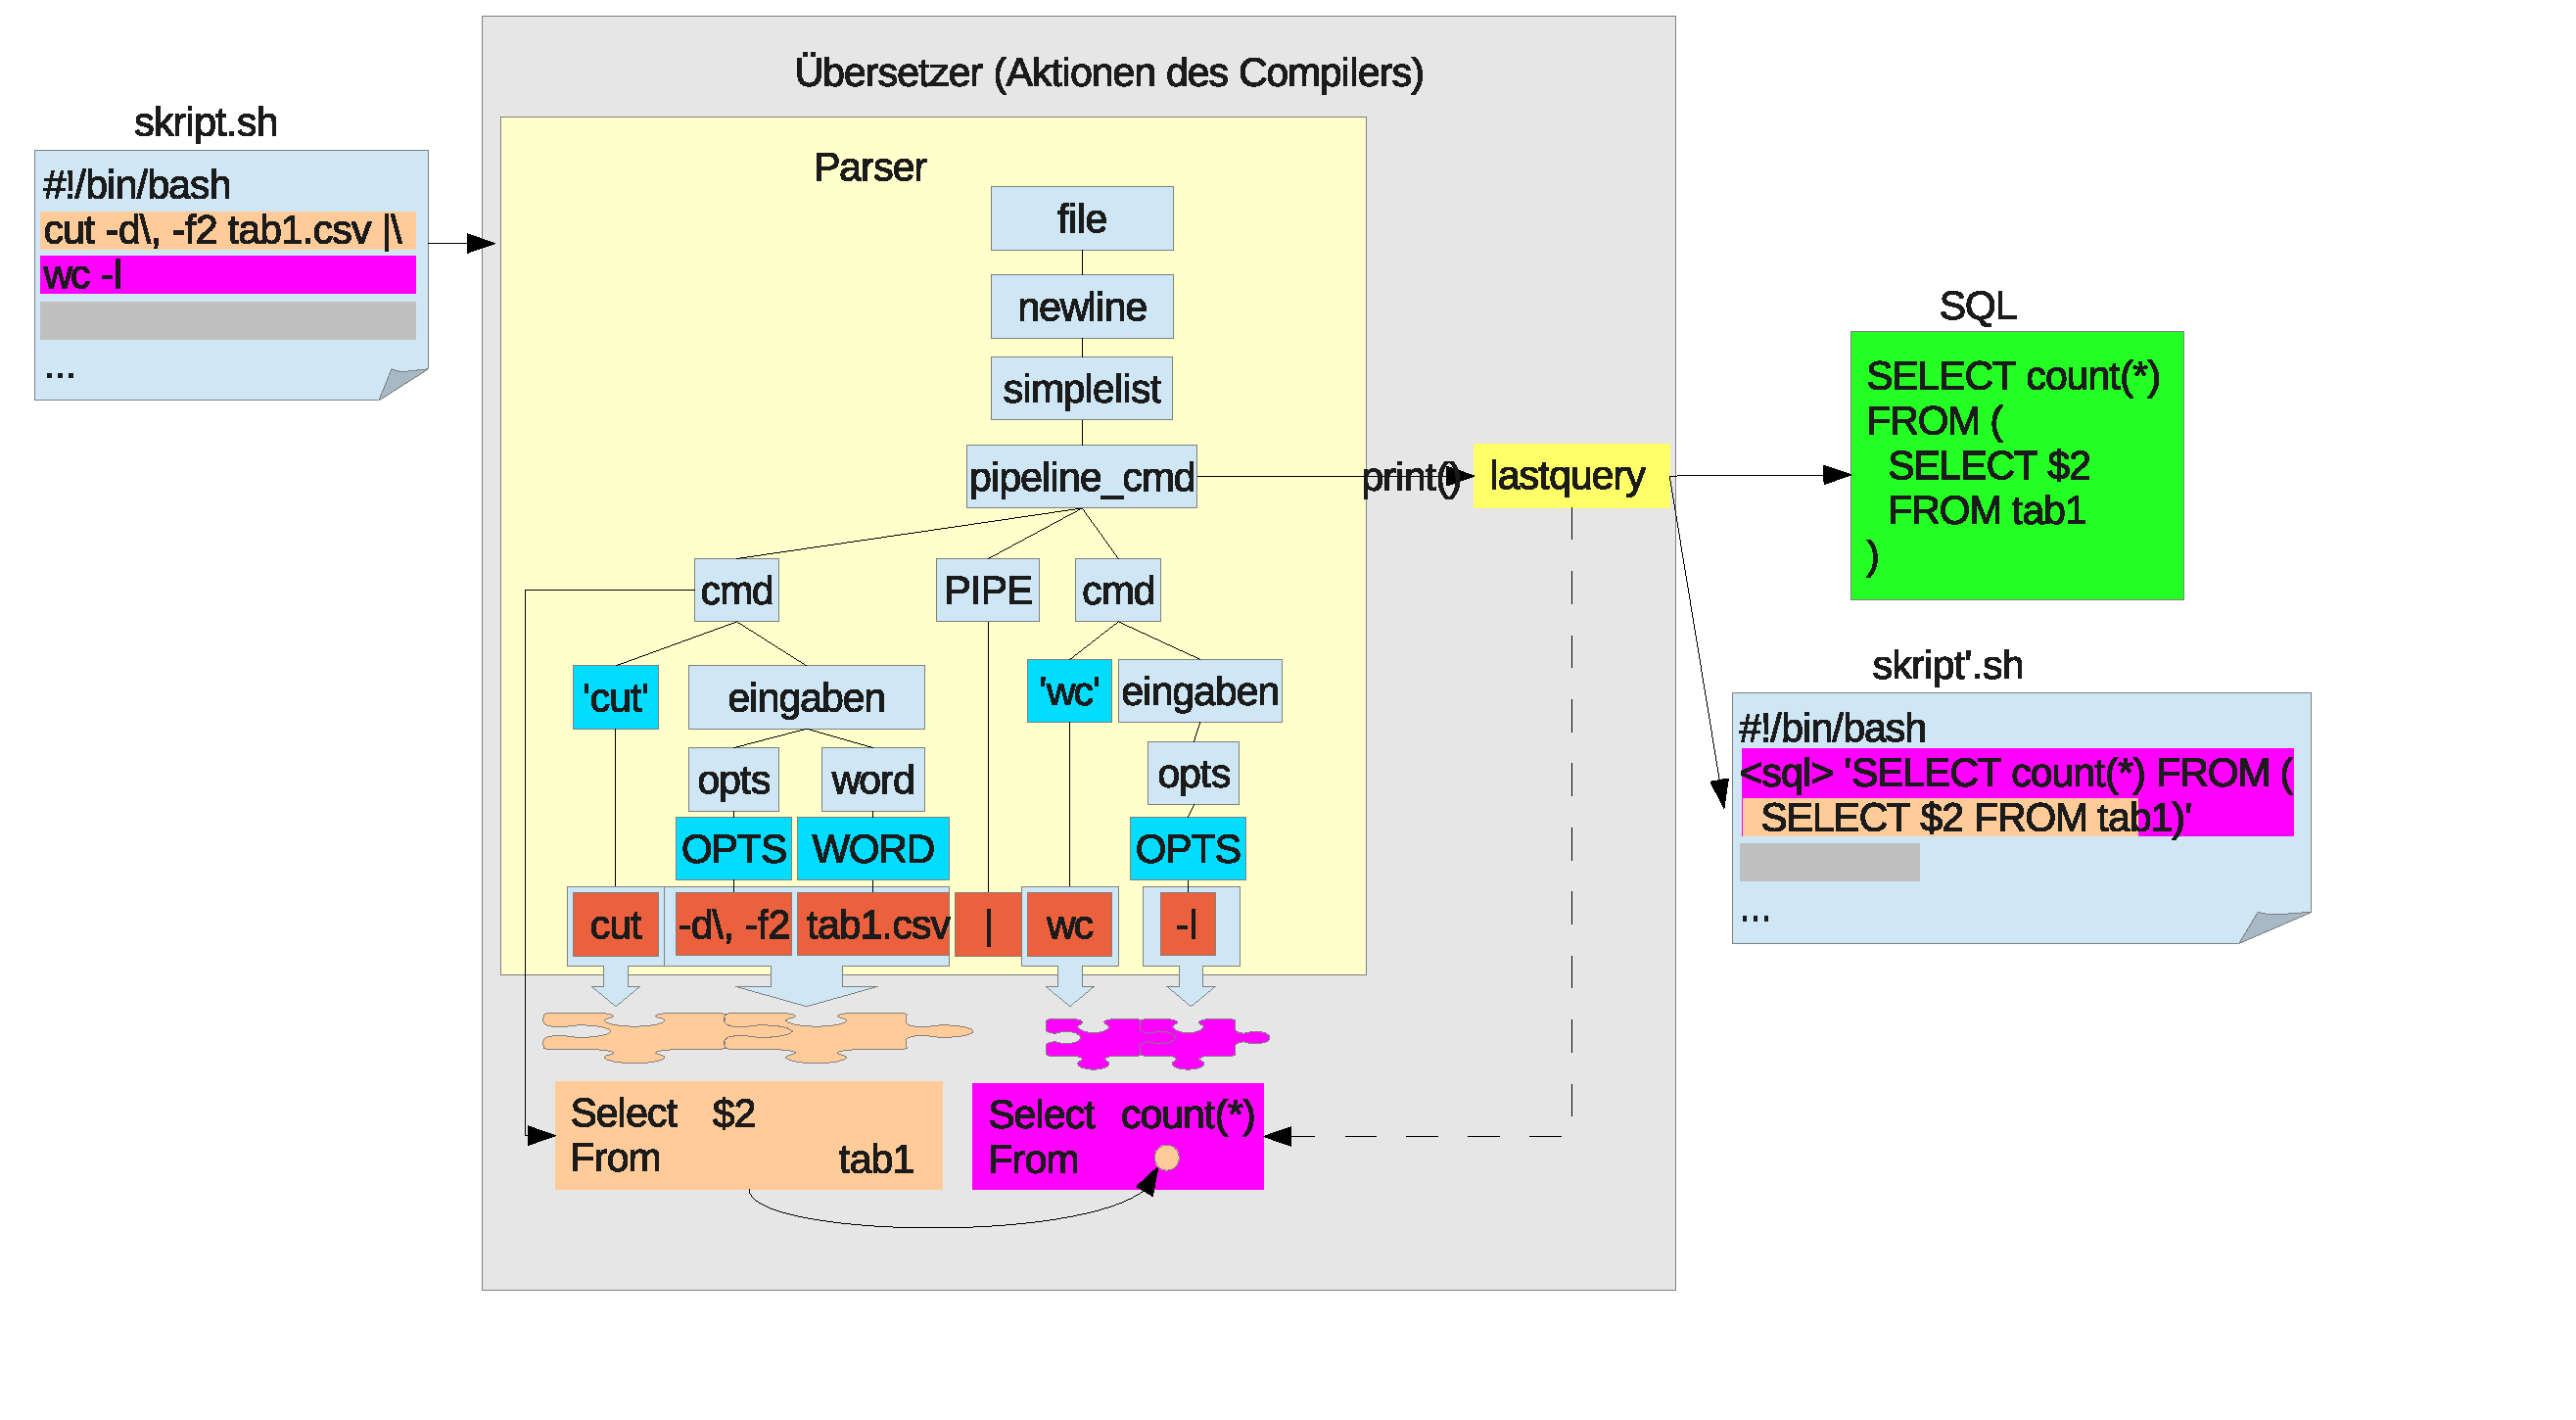
\includegraphics[scale=.4]{parsen_improve.eps}
\caption{Vorheriges Zusammenführen der Befehle}
\label{fig:improve}
\end{figure}

\section{Fazit}
Insgesamt ist es gelungen einen Vergleich aufzustellen, der die Laufzeit von Bash-Skripten analysiert. Es gibt einen Weg, die Abfragen zu übersetzen, und noch genug Platz für Ideen, um alle möglichen Skripte übersetzen zu können.
Diese Arbeit hat gezeigt, dass sich der Umstieg auf SQL lohnt, und will ermutigen, diesen Weg weiter zu verfolgen.
